\section{Conclusion}

\subsubsection{Future Work}

\paragraph{Neural Networks} We would hope to explore using neural networks
more. Ideally, we hope to develop on our research with Gabor filters and experiment
with Boltzmann machines to gradually develop a convolution neural network \cite{yannle, yannle2}.
We plan to continue development, with the repository continuing to be
updated on github.

\paragraph{Character Location} One benefit of 
correlation filters we were unable to test is their 
ability to provide the locations of the categorizations. 
This would be done by correlating the input data with the 
filters in the position domain, essentially allowing the filter 
to iterate across a larger image. Ideally, the results would 
yield a correlation energy plane with peaks signifying the location 
and class of each character, removing the need for the 
segmentation portion of pre-processing.

\paragraph{Correlation Filter Optimizations} Additionally, 
there is still much that can be done to optimize our 
correlation filters. We would like to improve our PSR 
algorithm to compute a smaller sidelobe and test various 
sizes to find the most accurate and robust area around the 
peak. Further, we can still optimize the correlation filter 
categorization process as a whole, generating a larger number 
of filters with training data to account for more characters, 
different fonts and rotation, and better noise handling. Because 
the correlation filters did not take long to train, we anticipate 
that adding fonts would not too greatly increase the time required 
to generate the filters; however, it would be interesting to compare 
the time and power necessary for the correlation filters to approach 
the versatility of other OCR methods.

\paragraph{Translation} While we were unable to get the 
translation portion of the project completed, it remains 
a critical step in our original project idea. As such, 
we would intend to resolve the issues we ran into previously 
and make the translation a working part of the post-processing section.


\subsubsection{Semester Schedule \& Work Distribution}
\begin{figure}[!]
		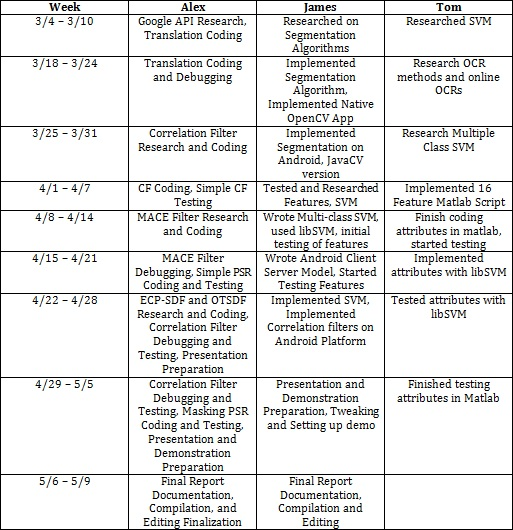
\includegraphics[scale=1.00]{schedule.jpg}\\
		\caption{Schedule of work done over semester}
		\label{fig:sch}
\end{figure}

\begin{figure}[!]
		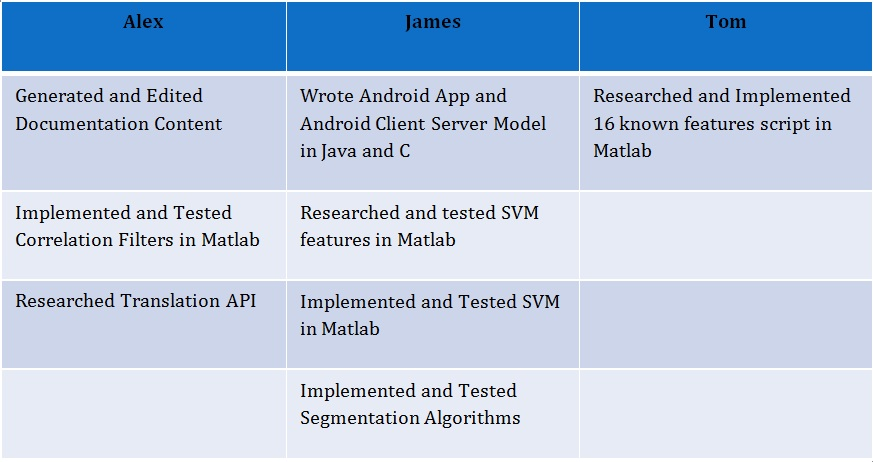
\includegraphics[scale=0.75]{work.jpg}\\
		\caption{Final Distribution of Work and Responsibilities}
		\label{fig:work}
\end{figure}